\chapter{اجزای مورد استفاده در سیستم ردیابی}
%\thispagestyle{empty}

\section{مقدمه}
هدف اصلی پروژه ما طراحی و پياده‌سازی سامانه‌ای است كه بتوان توسط آن موقعيت دقيق و مسير
حركت هر جسم متحرك را در هر زمان تعيين كرد. سامانه ذکر شده باید علاوه بر عملکرد مناسب، از لحاظ هزینه هم به صرفه باشد.


برای این که بتوانیم چنین سامانه‌ای را طراحی کنیم اول باید نیازمندی‌های سامانه را تشخیص دهیم، معماری کلی سامانه موردنظر خود را به دست آوریم و سپس با استفاده از این معماری و نیازسنجی انجام شده برای پیاده‌سازی از ماژول‌های مناسب استفاده کنیم. در این فصل در قسمت ۳-۲ ابتدا طرح کلی سامانه ردیابی را توضیح می‌دهیم و سپس در بخش ۳-۳ اجزاء مورد استفاده در این طرح را معرفی می‌کنیم.
\section{طراحی و معماری سیستم}
در اين پروژه قصد داريم به ساخت يک سيستم رديابي بپردازيم كه قادر است موقعيت دقيق و مسير حركت يک شي متحرك را مشخص كند. در انجام اين پروژه ارتباط ما به صورت يک طرفه خواهد بود به اين صورت كه به طور پيوسته مختصات مکاني شي متحرك توسط ماژول
 جی پی اس
 \RTLfootnote{\lr{GPS: Global Positioning System}}
  اندازه گرفته ميشود و به يک سرور فرستاده ميشود. اين ماژول به طور پيوسته با ماهواره برای گرفتن مختصات مکاني در ارتباط است. دادههای GPS به آردوينو فرستاده مي‌شود. در نهايت مودم GSM 3 اين اطلاعات را برای سرورهای
نرم‌افزاری ارسال مي‌كند. در اين پروژه سرورهای نرمافزاری پس از دريافت اطلاعات، آنها را تحليل ميكنند و درخواستي از سمت سرور نخواهيم داشت و ارتباط ما به صورت يکطرفه خواهد بود. در اين قسمت پروژه يک نرم‌افزار تحت وب توسعه داده خواهد شد تا
بتواند اطلاعات ارسالي را پردازش كرده و سپس آنها را در يک پايگاه داده ذخيره كند و در انتها اطلاعات ذخيره شده را به صورت قابل نمايش برای كاربران تبديل كند. هدف اصلي از انجام اين پروژه اين است كه مسير حركت شي متحرك را بر روی نقشه نشان
دهيم.
\verb;chapter1;
\section{اجزاء سیستم}
در قسمت قبل معماري سيستم را مشخص كرديم. حال اجزاء اين معماري را به طور دقيق بيان و معرفي می‌کنیم.
\subsection{اجزاء سخت‌افزاری}
اجزای سخت‌افزاری که برای پیاده‌سازی این سامانه استفاده شده است عبارتند از:
\begin{itemize}
	\item
	ماژول آردوینو
	\item
ماژول سیم ۸۰۸
\RTLfootnote{\lr{SIM 808}}
	\item
	آنتن جی پی اس
	\RTLfootnote{\lr{GPS Antenna}}
	\item
	آنتن جی اس ام
	\RTLfootnote{\lr{GSM Antenna}}
\end{itemize}
\subsection{ماژول آردوینو}
آردوينو يک ريزپردازنده متن‌باز اس كه براي نوشتن برنامه‌هايي كه با محیط و اشیا بیرون در تعامل هستند مناسب است. این برد مناسب نمونه‌سازی می‌باشد و نرم افزار و طرح سخت‌افزار آن به صورت آزاد در اختیار تمام افراد قرار گرفته است و هر فرد علاقه‌مند حتی با دانش و تجربه اندک در حوزه الکترونیک مي‌تواند از آردوینو برای انجام پروژه‌های خود استفاده نماید.


آردوينو محیط ساده‌ای براي برنامه‌نويسي دارد كه هر شخصي با اندكي آشنایی با زبان \lr{C} و  \lr{C++} مي‌تواند در این محیط برنامه‌نويسي كند و برنامه نوشته شده را در آردوینو اجرا نماید. به ميكروكنترلر آردوينو ميتوان حسگرهاي مختلف متصل و آن‌ها را كنترل كرد. ریزپردازنده به‌ کار رفته بر روی برد آردوینو بر اساس زبان برنامه‌نویسی آردوینو بر پایه \lr{Wiring} و محیط ویژه کدنویسی آن بر پایه \lr{Processing }برنامه‌ریزی شده است و برای کدنویسی به نرم‌افزار یا کامپایلر جانبی نیازی ندارد. 


آردوينو انواع مختلفي دارد كه ما از آردوینو \lr{Uno R3 } در این پروژه استفاده کرده‌ایم. \lr{R3} سومین و آخرین نسخه آردوینو \lr{Uno} می‌باشد. برد آردوینو \lr{Uno} یک میکروکنترلر بر پایه \lr{ATmega328} می‌باشد. ولتاژ كاري آن ۵ ولت مي‌باشد. ولتاژ ورودي این برد می‌تواند در بازه ۷ تا ۲۰ ولت باشد. این برد داراي ۶ پین ورودی آنالوگ، ۱۴ پين ورودي و خروجی ديجيتال، یک پورت یو اس \RTLfootnote{\lr{USB Port}}، یک ورودی منبع تغذیه و یک دکمه بازنشانی \RTLfootnote{\lr{Reset}} است که اجازه اتصال بردهای توسعه مختلفی را فراهم می‌آورد. در شكل ۳-۱ برد آردوينو \lr{Uno} را مشاهده مي‌كنيد.
\begin{figure}[!h]
	\centerline{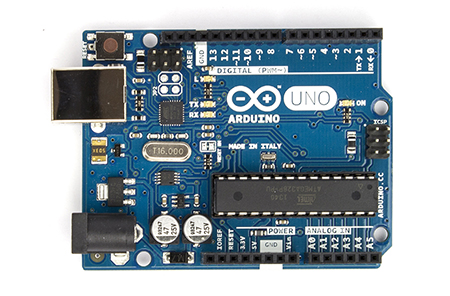
\includegraphics[width=.5\textwidth]{ArduinoUno_R3}}
	\caption{برد آردوینو \lr{UNO R3}}
\end{figure}

\subsection{اجزاء نرم‌افزاری}

\section{رعایت قواعد نشانه‌گذاری}
منظور از نشانه‌گذاري به‌کار‌بردن علامت‌ها و نشانه‌هايي است که خواندن و فهم درست یک جمله را ممکن و آسان مي‌کند. در ادامه نشانه‌هاي معمول و متداول در زبان فارسي و موارد کاربرد آنها به اختصار معرفی می‌شوند.

\subsection{ويرگول}
ويرگول نشانه ضرورت یک مکث کوتاه است و در موارد زير به‌کار مي‌رود:
\begin{itemize}
\item
در ميان دو کلمه که احتمال داده شود خواننده آنها را با کسره اضافه بخواند، يا نبودن ويرگول موجب بروز اشتباه در خواندن جمله شود.
\item
در موردي که کلمه يا عبارتي به‌‌‌‌عنوان توضيح، در ضمن یک جمله آورده شود. مثلاً برای کنترل وضعیت فضاپیماها، به‌دلیل آن‌که در خارج از جو هستند، نمی‌توان از بالک‌های آیرودینامیکی استفاده کرد.
\item
جدا‌کردن بخش‌هاي مختلف يک نشاني يا یک مرجع
\item
موارد دیگر از این قبیل
\end{itemize}
پیش از ويرگول نبايد فاصله گذاشته شود و پس از آن يک فاصله لازم است و بيشتر از آن صحیح نیست.
\subsection{نقطه}
نقطه نشانه پایان یک جمله است. پیش از نقطه نبايد فاصله گذاشته شود و پس از آن يک فاصله لازم است و بيشتر از آن صحیح نیست.
\subsection{دونقطه}
موارد کاربرد دونقطه عبارتند از:
\begin{itemize}
\item
پيش از نقل قول مستقيم
\item
پيش از بيان تفصيل مطلبي که به اجمال به آن اشاره شده‌است.
\item
پس از واژه‌اي که معني آن در برابرش آورده و نوشته مي‌شود.
\item
پس از کلمات تفسير‌کننده از قبيل «يعني» و ...
\end{itemize}
پیش از دونقطه نبايد فاصله گذاشته شود و پس از آن يک فاصله لازم است و بيشتر از آن صحیح نیست.
\subsection{گیومه}
موارد کاربرد گیومه عبارتند از:
\begin{itemize}
\item
وقتي که عين گفته يا نوشته کسي را در ضمن نوشته و مطلب خود مي‌آوريم. 
\item
در آغاز و پايان کلمات و اصطلاحات علمي و يا هر کلمه و عبارتي که بايد به‌صورت ممتاز از قسمت‌هاي ديگر نشان داده شود.
\item
در ذکر عنوان مقاله‌ها، رساله‌ها، اشعار، روزنامه‌ها و ...
\end{itemize}
\subsection{نشانه پرسشی}
پیش از «؟» نبايد فاصله گذاشته شود و پس از آن يک فاصله لازم است و بيشتر از آن صحیح نیست.
\subsection{خط تیره}
موارد کاربرد خط تیره عبارتند از:
\begin{itemize}
\item
جدا‌کردن عبارت‌هاي توضيحي، بدل، عطف بيان و ...
\item
به‌جاي حرف اضافه «تا» و «به» بين تاريخ‌ها، اعداد و کلمات
\end{itemize}
\subsection{پرانتز}
موارد کاربرد پرانتز عبارتند از:
\begin{itemize}
\item
به‌معني «يا» و «يعني» و وقتي که یک کلمه يا عبارت را براي توضيح بيشتر کلام بياورند.
\item
وقتي که نويسنده بخواهد آگاهي‌هاي بيشتر (اطلاعات تکميلي) به خواننده عرضه کند.
\item
براي ذکر مرجع در پايان مثال‌ها و شواهد.
\end{itemize}
نکته: بین کلمه یا عبارت داخل پرانتز و پرانتز باز و بسته نباید فاصله وجود داشته باشد.
\section{جدا یا سرهم نوشتن برخی کلمات}
تقريباً تمامي کلمات مرکب در زبان فارسي بايد از هم جدا نوشته شوند؛ به استثناي صفات فاعلي مانند «عملگر»، «باغبان» و يا «دانشمند» و کلماتي نظير «اينکه»، «آنها». در ادامه به نمونه‌هايي از مواردي که بايد اجزاي يک کلمه جدا، اما بدون فاصله نوشته شوند، اشاره مي‌شود‌:
\begin{enumerate}
\item
در افعال مضارع و ماضی استمراری که با «می» شروع می‌شوند، لازم است که در عين جدا نوشتن، «می» از بخش بعدي فعل جدا نيافتد‌.‌ برای اين منظور بايد از «فاصله متصل» استفاده و «می» در اول فعل با \lr{SS}\LTRfootnote{Shift+Ctrl+@} از آن جدا شود.‌ به‌طور مثال «می‌شود» به‌جاي «می شود». 
\item
	«ها»ی جمع بايد از کلمه جمع بسته‌شده جدا نوشته شود؛ مگر در برخی کلمات مانند «آنها». اين امر در مورد کلمات غير‌فارسي که وارد زبان فارسي شده‌اند و با حرف «ها» جمع بسته می‌شوند، مانند «کانال‌ها» يا «فرمول‌ها» مورد تاکيد است.
\item
	حروف اضافه مانند «به» وقتي به‌صورت ترکيب ثابت همراه کلمه پس از خود آورده می‌شوند، بهتر است با \lr{SS} از آن جدا شوند‌.‌ مانند «به‌صورت»، «به‌عنوان» و «به‌‌‌لحاظ»‌.‌ لازم به ذکر است هنگامی که حرف اضافه «به» با کلمه پس از خود معناي قيدي داشته باشد، مثل «بشدت» يا «بسادگي»، بهتر است که به‌صورت چسبيده نوشته شود‌.
\item
	کلمات فارسی نبايد با قواعد عربی جمع بسته شوند؛ پس «پيشنهادها» صحيح و «پيشنهادات» اشتباه است‌.‌
\item
	اسم‌ها و صفت‌هاي دو‌قسمتي مثل «خط‌چين» و «نوشته‌شده» با \lr{SS} از هم جدا می‌شود‌.‌
\item
	شناسه‌ها با \lr{SS} از کلمه اصلي جدا می‌شود‌.‌ مثل «شده‌اند»‌ و «شده‌است». 
\item
	‌ «است» هنگامی که نقش شناسه را داشته باشد توسط \lr{SS} از قسمت اصلي جدا می‌شود‌.‌ مانند «گفته‌است»‌.
\item
	بند پیشین نبايد باعث افراط در استفاده از فاصله متصل شود. مثلاً عبارت «نوشته می‌شود‌« صحيح و عبارت «نوشته‌می‌شود» ناصحیح است. 
\item
	فعل‌هاي دو‌کلمه‌اي که معناي اجزاي آنها کاملاً با معناي کل متفاوت است، بهتر است که با \lr{SS} از هم جدا ‌شوند‌.‌
\item
	کلمات مرکب مثل کلمه «دوکلمه‌اي» در عبارت «فعل‌هاي دوکلمه‌اي» و «يادداشت‌برداري».
\item
	مصدرهاي دو قسمتي با \lr{SS} از هم جدا می‌شوند‌.‌ مثل «ذوب‌کردن» و «واردکردن»‌.
\item
	 صفات تفضيلي مثل « آسان‌تر».
\end{enumerate}

